\subsection{Einfacher Common-Emitter-Verstärker} % (fold)
\label{sub:Einfacher_Common-Emitter-Verstärker}
\begin{frame}
    \frametitle{Einfacher Common-Emitter-Verstärker}
    \framesubtitle{}
    \begin{figure}[H]
    \begin{center}
            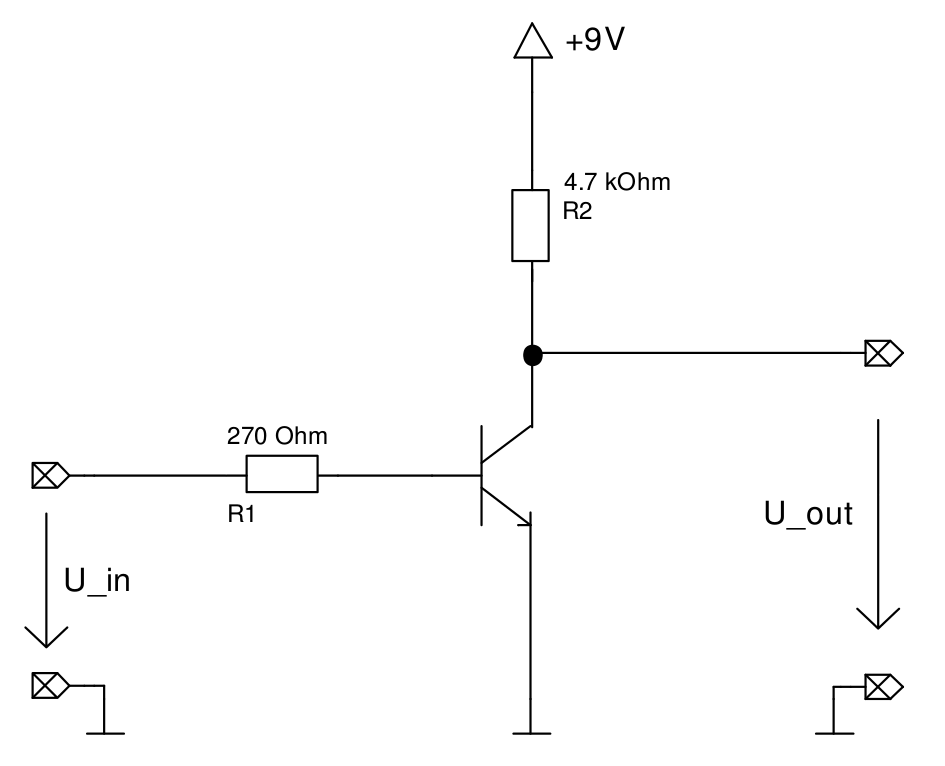
\includegraphics[scale=0.2]{./img/schaltungen/common_emitter_einfach.png}
    \end{center}
    \end{figure}
\end{frame}
\begin{frame}
    \frametitle{Einfacher Common-Emitter-Verstärker}
    \framesubtitle{}
     \begin{columns}[c]
     \column{0.4\textwidth}
        \begin{figure}[H]
        \begin{center}
                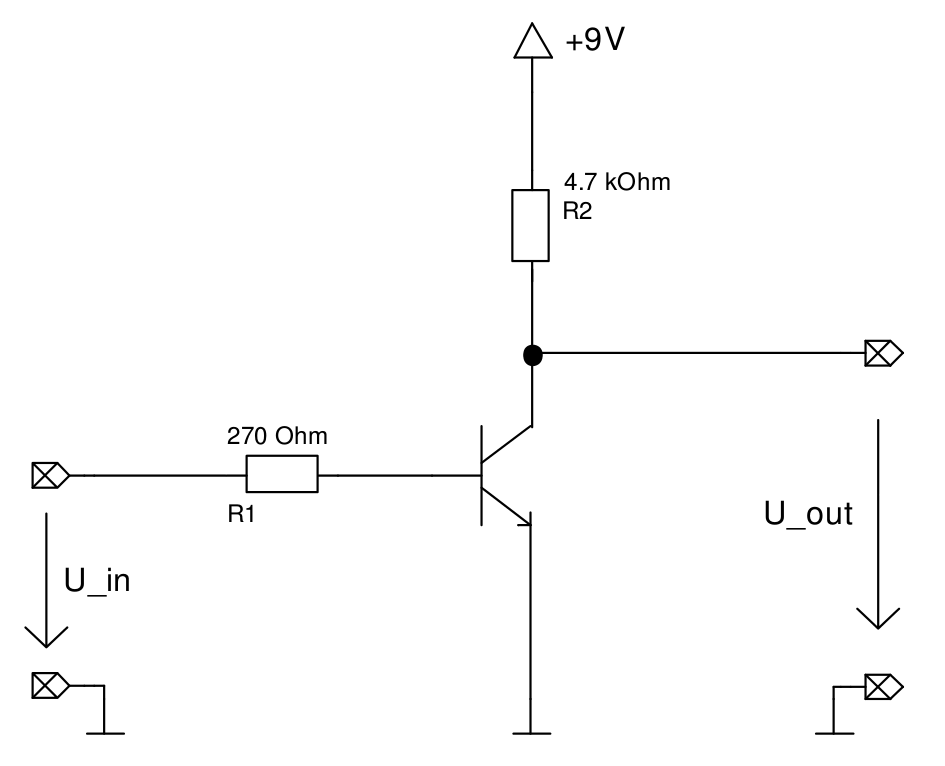
\includegraphics[scale=0.16]{./img/schaltungen/common_emitter_einfach.png}
        \end{center}
        \end{figure}
     \column{0.4\textwidth}
         \begin{block}{Funktionsprinzip}
            \begin{itemize}
                \item Wechselspannung wird an $U_{in}$ angelegt
                \item Spannung $U_{out}$ ist konstant
                \item übersteigt $U_{in}$ die Transistor-Schwellspannung wird
                der Transistor durchgeschaltet
                \item Fast kein Spannungsabfall zwischen Kollektor und Masse
                $\rightarrow$ $U_out$ fällt stark ab
            \end{itemize}    
         \end{block}
     \end{columns}
\end{frame}
\begin{frame}
    \frametitle{Einfacher Common-Emitter-Verstärker}
    \framesubtitle{}
    \begin{columns}[c]
    \column{0.4\textwidth}
        \begin{figure}[H]
        \begin{center}
                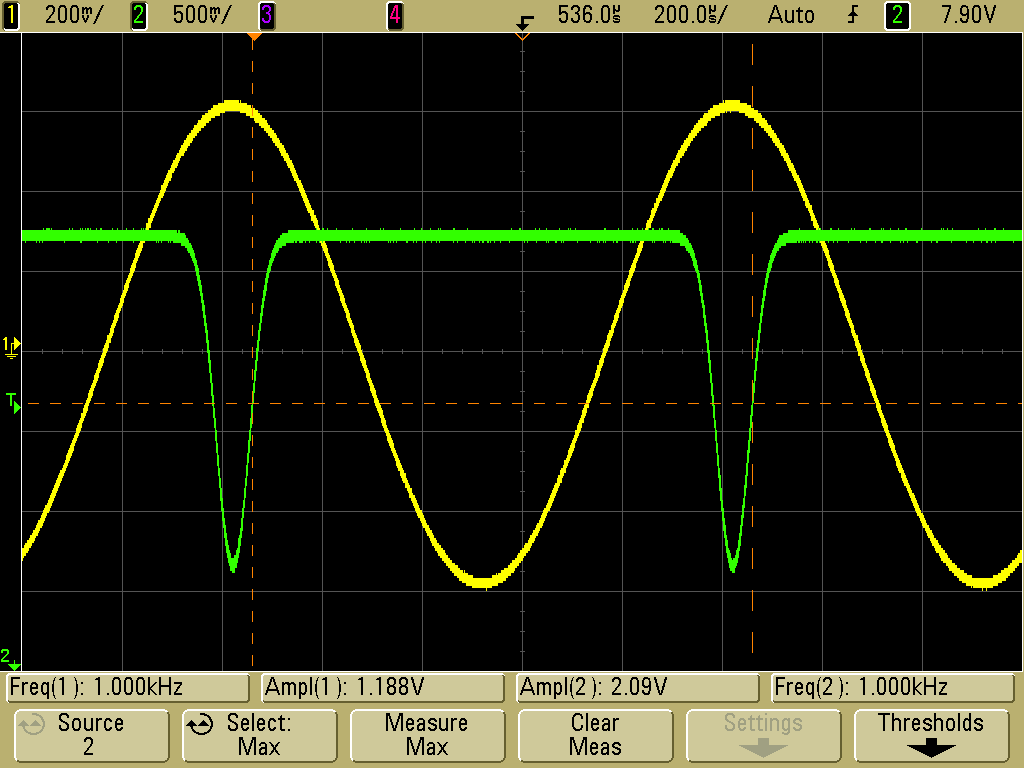
\includegraphics[scale=0.15]{./img/oszi/Aufgabe31.png}
        \end{center}
        \end{figure}
    \column{0.4\textwidth}
        \begin{block}{Funktionsprinzip}
            \begin{itemize}
                \item Wechselspannung wird an $U_{in}$ angelegt
                \item Spannung $U_{out}$ ist konstant
                \item übersteigt $U_{in}$ die Transistor-Schwellspannung wird
                der Transistor durchgeschaltet
                \item Fast kein Spannungsabfall zwischen Kollektor und Masse
                $\rightarrow$ $U_{out}$ fällt stark ab
            \end{itemize}    
         \end{block}
    \end{columns}
\end{frame}
\begin{frame}
    \frametitle{Einfacher Common-Emitter-Verstärker}
    \framesubtitle{}
     \begin{columns}[c]
        \column{0.4\textwidth}
        \begin{figure}[H]
        \begin{center}
                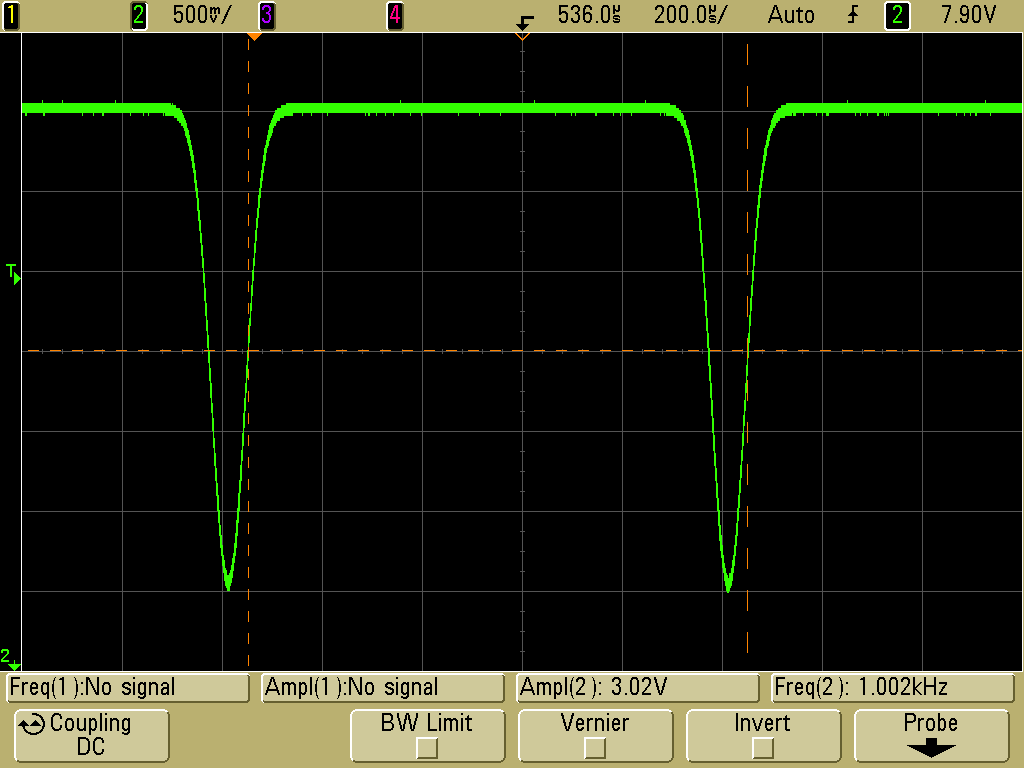
\includegraphics[scale=0.15]{./img/oszi/Aufgabe31_finger.png}
        \end{center}
        \end{figure}
        \column{0.4\textwidth}
        \begin{block}{}
            \begin{itemize}
                \item Berühren des Transistors verstärkt Abfall
                \item Erklärung: Geringerer Spannungsabfall an Transistor durch
                Berühren
            \end{itemize}
        \end{block}
     \end{columns}
\end{frame}
